\documentclass[12pt, titlepage]{article}

\usepackage{fullpage}
\usepackage[round]{natbib}
\usepackage{multirow}
\usepackage{booktabs}
\usepackage{tabularx}
\usepackage{graphicx}
\usepackage{float}
\usepackage{hyperref}
\usepackage{pdfpages}

\hypersetup{
    colorlinks,
    citecolor=black,
    filecolor=black,
    linkcolor=red,
    urlcolor=blue
}
\usepackage[round]{natbib}

\newcounter{acnum}
\newcommand{\actheacnum}{AC\theacnum}
\newcommand{\acref}[1]{AC\ref{#1}}

\newcounter{ucnum}
\newcommand{\uctheucnum}{UC\theucnum}
\newcommand{\uref}[1]{UC\ref{#1}}

\newcounter{mnum}
\newcommand{\mthemnum}{M\themnum}
\newcommand{\mref}[1]{M\ref{#1}}

\title{SE 3XA3: Software Requirements Specification\\Snake 2.0}

\author{Team \#34, Send Help 
		\\ George Mo (moz)
		\\ Harrison Lau (lauh3)
		\\ Vanessa Truong(truonv1)
}

\date{\today}

\begin{document}

\maketitle

\pagenumbering{roman}
\tableofcontents
\listoftables
\listoffigures

\begin{table}[bp]
\caption{\bf Revision History}
\begin{tabularx}{\textwidth}{p{3cm}p{2cm}X}
\toprule {\bf Date} & {\bf Version} & {\bf Notes}\\
\midrule
Nov 10, 2017 & 1.0 & Finished Sections 1, 2, 3\\
Nov 10 & 1.1 & Finished Sections 4, 5, 6, 7, 8\\
Dec 2 & 2.0 & Final revision - Added Scoreboard module and updated uses hierarchy\\
\bottomrule
\end{tabularx}
\end{table}

\newpage

\pagenumbering{arabic}

\section{Introduction}

\subsection{Purpose}

Our project purpose is to reimplement the classic arcade game, Snake, by adding newly designed features that will add a modern flair to the gameplay. 
Snake 2.0 will encompass Snake's basic functionality along with some twists to the game which will include map changes, power-ups and an enhanced GUI.

\subsection{Overview}

This document will specify the modular structure and decomposition of our reimplementation, and will serve as the Module Guide (MG) for our project. The decomposition will follow the design principles of information hiding and encapsulation, and the uses hierarchy, as they allow great flexibility for potential changes to our modules. With the basis of these principles, our modular design will abide by the following rules:

\begin{itemize}
\item Details in our modules with prospects of change will be kept private to that respective module. 
\item Any changes to the module "secrets" (anticpated changes) will not change the module design interface.
\item There will be a lenience towards low-coupling and high cohesion within the modules.
\item The uses relation between modules will encompass a "fan-in" characteristic.
\end{itemize}

The MG is intended to be easily understood by all project members, for efficient maintenance and design, and should be easy to follow for the course instructors and assistants. Having the module guide follow a hierarchical structure will provide project members with a better understanding of the modules when changes need to be implemented.\\

The rest of the document is organized as follows:
\begin{itemize}
\item Section \ref{SecChange} lists the anticipated and unlikely changes of the software requirements. 
\item Section \ref{SecMH} summarizes the module decomposition that was constructed according to the likely changes. 
\item Section \ref{SecConnection} specifies the connections between the software requirements and the modules. 
\item Section \ref{SecMD} gives a detailed description of the modules. 
\item Section \ref{SecTM} includes two traceability matrices. One checks the completeness of the design against the requirements provided in the SRS. The
other shows the relation between anticipated changes and the modules. 
\item Section \ref{SecUse} describes the use relation between modules.
\end{itemize}

\section{Anticipated and Unlikely Changes} \label{SecChange}

This section highlights the possible changes that may be made to Snake 2.0. According to the likeliness
of the change, the possible changes are classified into two
categories; anticipated changes (Section \ref{SecAchange}), and
unlikely changes (Section \ref{SecUchange}).

\subsection{Anticipated Changes} \label{SecAchange}

Anticipated changes are the source of the information that is to be hidden
inside the modules. Ideally, changing one of the anticipated changes will only
require changing the one module that hides the associated decision. The approach
adapted here is called design for change. The following lists the anticpated changes to the module design:

\begin{description}
\item[\refstepcounter{acnum} \actheacnum \label{acMapChanges}:] The options for in-game map changes (i.e. what mape sizes to incorporate)
\item[\refstepcounter{acnum} \actheacnum \label{acSpeedUp}:] The numeric scale to which a pellet increases the Snake's speed.
\item[\refstepcounter{acnum} \actheacnum \label{acSpeedDown}:] The numeric scale to which a pellet decreases the Snake's speed.
\item[\refstepcounter{acnum} \actheacnum \label{acBoundaryCollision}:] The length of time for which invincibility to boundary collision will last.
\item[\refstepcounter{acnum} \actheacnum \label{acSelfCollision}:] The length of time for which invinicibility to self-collision will last.
\item[\refstepcounter{acnum} \actheacnum \label{acAdditional}:] Additional in-game features (e.g. move keys produce unexpected Snake direction)
\item[\refstepcounter{acnum} \actheacnum \label{acMenuGUI}:] The graphical user interface design for the menu.
\item[\refstepcounter{acnum} \actheacnum \label{acHardware}:] The prospect of other platform compabilities (e.g. mobile, web)
\end{description}

\subsection{Unlikely Changes} \label{SecUchange}

Although module design is more favourable when it is as general as possible, complexity is proportional to the generality of the module design. Thus, once design decisions are being simplified, other parts of the design will also require changes. The following decisions that are listed will not be changed:

\begin{description}
\item[\refstepcounter{ucnum} \uctheucnum \label{ucIO}:] Input/Output devices to the game (Game will assume keyboard and monitor is available).
\item[\refstepcounter{ucnum} \uctheucnum \label{ucInput}:] The arrow keys for dictating Snake's movement.
\item[\refstepcounter{ucnum} \uctheucnum \label{ucBasic}:] The basic functionality of the original Snake game will be retained (i.e. eating pellets, growing in size, avoiding collisions)
\item[\refstepcounter{ucnum} \uctheucnum \label{ucScore}:] There will always be an in-game scoreboard to track player's score.
\end{description}

\section{Module Hierarchy} \label{SecMH}

This section provides an overview of the module design. Modules are summarized
in a hierarchy decomposed by secrets in Table \ref{TblMH}. The modules listed
below, which are leaves in the hierarchy tree, are the modules that will
actually be implemented.

\begin{description}
\item [\refstepcounter{mnum} \mthemnum \label{mHH}:] Hardware-Hiding Module
\item [\refstepcounter{mnum} \mthemnum \label{mSM}:] Snake Module
\item [\refstepcounter{mnum} \mthemnum \label{mMM}:] Menu Module
\item [\refstepcounter{mnum} \mthemnum \label{mBM}:] Board Module
\item [\refstepcounter{mnum} \mthemnum \label{mSBM}:] Scoreboard Module
\end{description}


\begin{table}[h!]
\centering
\begin{tabular}{p{0.3\textwidth} p{0.6\textwidth}}
\toprule
\textbf{Level 1} & \textbf{Level 2}\\
\midrule

{Hardware-Hiding Module} & ~ \\
\midrule

\multirow{3}{0.3\textwidth}{Behaviour-Hiding Module} & Scoreboard Module\\
& Menu Module\\
& Scoreboard Module\\
\midrule

\multirow{1}{0.3\textwidth}{Software Decision Module} & {Snake Module}\\
\bottomrule

\end{tabular}
\caption{Module Hierarchy}
\label{TblMH}
\end{table}

\section{Connection Between Requirements and Design} \label{SecConnection}

The design of the system is intended to satisfy the requirements developed in
the SRS. In this stage, the system is decomposed into modules. The connection
between requirements and modules is listed in Table \ref{TblRT}.

The Board module contains all of the in-game functional requirements, and the in-game non-functional requirements, exhibiting the roles of the controller and model in the MVC design pattern. It deals with the input and output functionalities, as well as the look and feel, usability, and performance requirements. Such requirements include the input/output of the arrow keys for moving the snake, the speed in which the Snake moves at, the colour choices for the in-game board, and the response time to user inputs. 

The Menu module will be the model and controller for the menu GUI. It will control all the design elements incorporated into the game's menu, such as the buttons and the different pages. The menu will essentially encompass a simplistic and colourful interface to satisfy the look and feels requirements, as well as the usability requirements. 

The Scoreboard module will be part of the model component. It will simply display the player's score at the bottom of the application window.

The Snake module plays the role of the view component, which connects all the modules together and generates the output for the user based on their inputs processed by the Board module and Menu module. 

\section{Module Decomposition} \label{SecMD}

The principle of ``information hiding'' proposed by \citet{ParnasEtAl1984} will be used as the basis 
for our module decomposition. The \emph{Secrets} field provides a brief statement of the design decision hidden by the
module. The \emph{Services} field specifies \emph{what} the module will do
without documenting \emph{how} to do it. For each module, a suggestion for the
implementing software is given under the \emph{Implemented By} title. 

The following is the list of modules that will be implemented, noting that only the leaf modules in the hierarchy require implementation. Modules 
that don't require implementation will be marked with a dash (-). 

\subsection{Hardware Hiding Modules (\mref{mHH})}

\begin{description}
\item[Secrets:]The data structure and algorithm used to implement the virtual
  hardware.
\item[Services:]Serves as a virtual hardware used by the rest of the
  system. This module provides the interface between the hardware and the
  software. It processes and communicates to the software all I/O actions from the hardware.
\item[Implemented By:] OS
\end{description}

\subsection{Behaviour-Hiding Module}

\begin{description}
\item[Secrets:]The contents of the required behaviours.
\item[Services:]Includes programs that provide externally visible behaviour of
  the system as specified in the software requirements specification (SRS)
  documents. This module serves as a communication layer between the
  hardware-hiding module and the software decision module. The programs in this
  module will need to change if there are changes in the SRS.
\item[Implemented By:] --
\end{description}

\subsubsection{Board Module (\mref{mBM})}

\begin{description}
\item[Secrets:]The set-up variables for the game (window size, snake directions, pellet position, etc.)
\item[Services:] Sets up all the game features and stores variables for controlling the game's objects.
\item[Implemented By:] Java Abstract Windows Toolkit and Swing Library
\end{description}

\subsubsection{Menu Module (\mref{mMM})}

\begin{description}
\item[Secrets:] Menu set-up
\item[Services:] Sets up the start-up game menu window, buttons, and pages
\item[Implemented By:] Java Abstract Windows Toolkit and Swing Library
\end{description}

\subsubsection{ScoreBoard Module (\mref{mSBM})}

\begin{description}
\item[Secrets:] The in-game scoreboard set-up 
\item[Services:] Sets up the player's score during in-game sate and game over state
\item[Implemented By:] Java Abstract Windows Toolkit and Swing Library
\end{description}

\subsection{Software Decision Module}

\begin{description}
\item[Secrets:] The design decision based on mathematical theorems, physical
  facts, or programming considerations. The secrets of this module are
  \emph{not} described in the SRS.
\item[Services:] Includes data structure and algorithms used in the system that
  do not provide direct interaction with the user. 
  Changes in these modules are more likely to be motivated by a desire to
  improve performance than by externally imposed changes.
\item[Implemented By:] --
\end{description}

\subsubsection{Snake Module (\mref{mSM})}

\begin{description}
\item[Secrets:] Format window and display
\item[Services:] Sets up game window and displays Board and Menu modules
\item[Implemented By:] Java Abstract Windows Toolkit and Swing Library
\end{description}

\section{Traceability Matrix} \label{SecTM}

This section shows two traceability matrices: between the modules and the
requirements and between the modules and the anticipated changes.

\begin{table}[H]
\centering
\begin{tabular}{p{0.2\textwidth} p{0.6\textwidth}}
\toprule
\textbf{Req.} & \textbf{Modules}\\
\midrule
\textbf{Functional Req.}\\
\midrule
FR1 & \mref{mHH}, \mref{mBM}\\
FR2 & \mref{mBM}\\
FR3 & \mref{mBM}\\
FR4 & \mref{mHH}, \mref{mBM}, \mref{mSM}, \mref{mMM}\\
FR5 & \mref{mBM}\\
FR6 & \mref{mBM}, \mref{mSBM}\\
FR7 & \mref{mSM}, \mref{mBM}, \mref{mMM}\\
\midrule
\textbf{Non-functional Req.}\\
\midrule
NFR1 & \mref{mMM}, \mref{mBM}\\
NFR2 & \mref{mMM}, \mref{mBM}\\
NFR3 & \mref{mHH}, \mref{mBM}, \mref{mSBM}\\
NFR4 & \mref{mHH}, \mref{mBM}\\
NFR5 & \mref{mMM}, \mref{mBM}\\
NFR6 & \mref{mHH}, \mref{mMM}, \mref{mBM}, \mref{mSM}\\
NFR7 & \mref{mHH}, \mref{mBM}\\
NFR8 & \mref{mHH}\\
NFR9 & \mref{mHH}, \mref{mMM}, \mref{mBM}, \mref{mSM}\\
NRF10 & \mref{mMM}, \mref{mBM}\\
NFR11 & \mref{mMM}\\
NRF12 & \mref{mMM}, \mref{mBM}\\
\bottomrule
\end{tabular}

\caption{Trace Between Requirements and Modules}
\label{TblRT}
\end{table}

\begin{table}[H]
\centering
\begin{tabular}{p{0.2\textwidth} p{0.6\textwidth}}
\toprule
\textbf{AC} & \textbf{Modules}\\
\midrule
\acref{acMapChanges} & \mref{mBM}, \mref{mSM}, \mref{mMM}\\
\acref{acSpeedUp} & \mref{mBM}\\
\acref{acSpeedDown} & \mref{mBM}\\
\acref{acBoundaryCollision} & \mref{mBM}\\
\acref{acSelfCollision} & \mref{mBM}\\
\acref{acAdditional} & \mref{mBM}\\
\acref{acMenuGUI} & \mref{mSM}, \mref{mMM}\\
\acref{acHardware} & \mref{mHH}\\
\bottomrule
\end{tabular}
\caption{Trace Between Anticipated Changes and Modules}
\label{TblACT}
\end{table}

\section{Use Hierarchy Between Modules} \label{SecUse}

In this section, the uses hierarchy between modules is
provided. \citet{Parnas1978} said of two programs A and B that A {\em uses} B if
correct execution of B may be necessary for A to complete the task described in
its specification. That is, A {\em uses} B if there exist situations in which
the correct functioning of A depends upon the availability of a correct
implementation of B.  Figure \ref{FigUH} illustrates the use relation between
the modules. It can be seen that the graph is a directed acyclic graph
(DAG). Each level of the hierarchy offers a testable and usable subset of the
system, and modules in the higher level of the hierarchy are essentially simpler
because they use modules from the lower levels.

\begin{figure}[H]
\centering
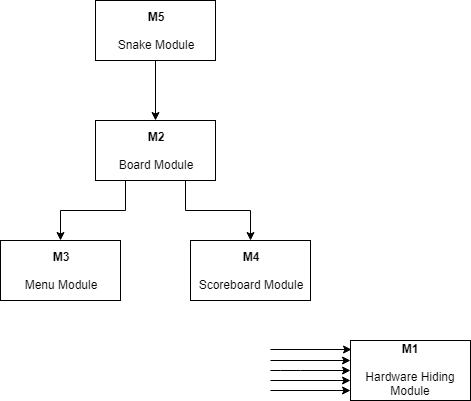
\includegraphics[width=1.0\textwidth]{UsesHierarchy.png}
\caption{Use hierarchy among modules}
\label{FigUH}
\end{figure}

\section{Gantt Chart}
\label{gantt}
The following pages include an updated Gantt Chart (updated in appropriate folder as well).
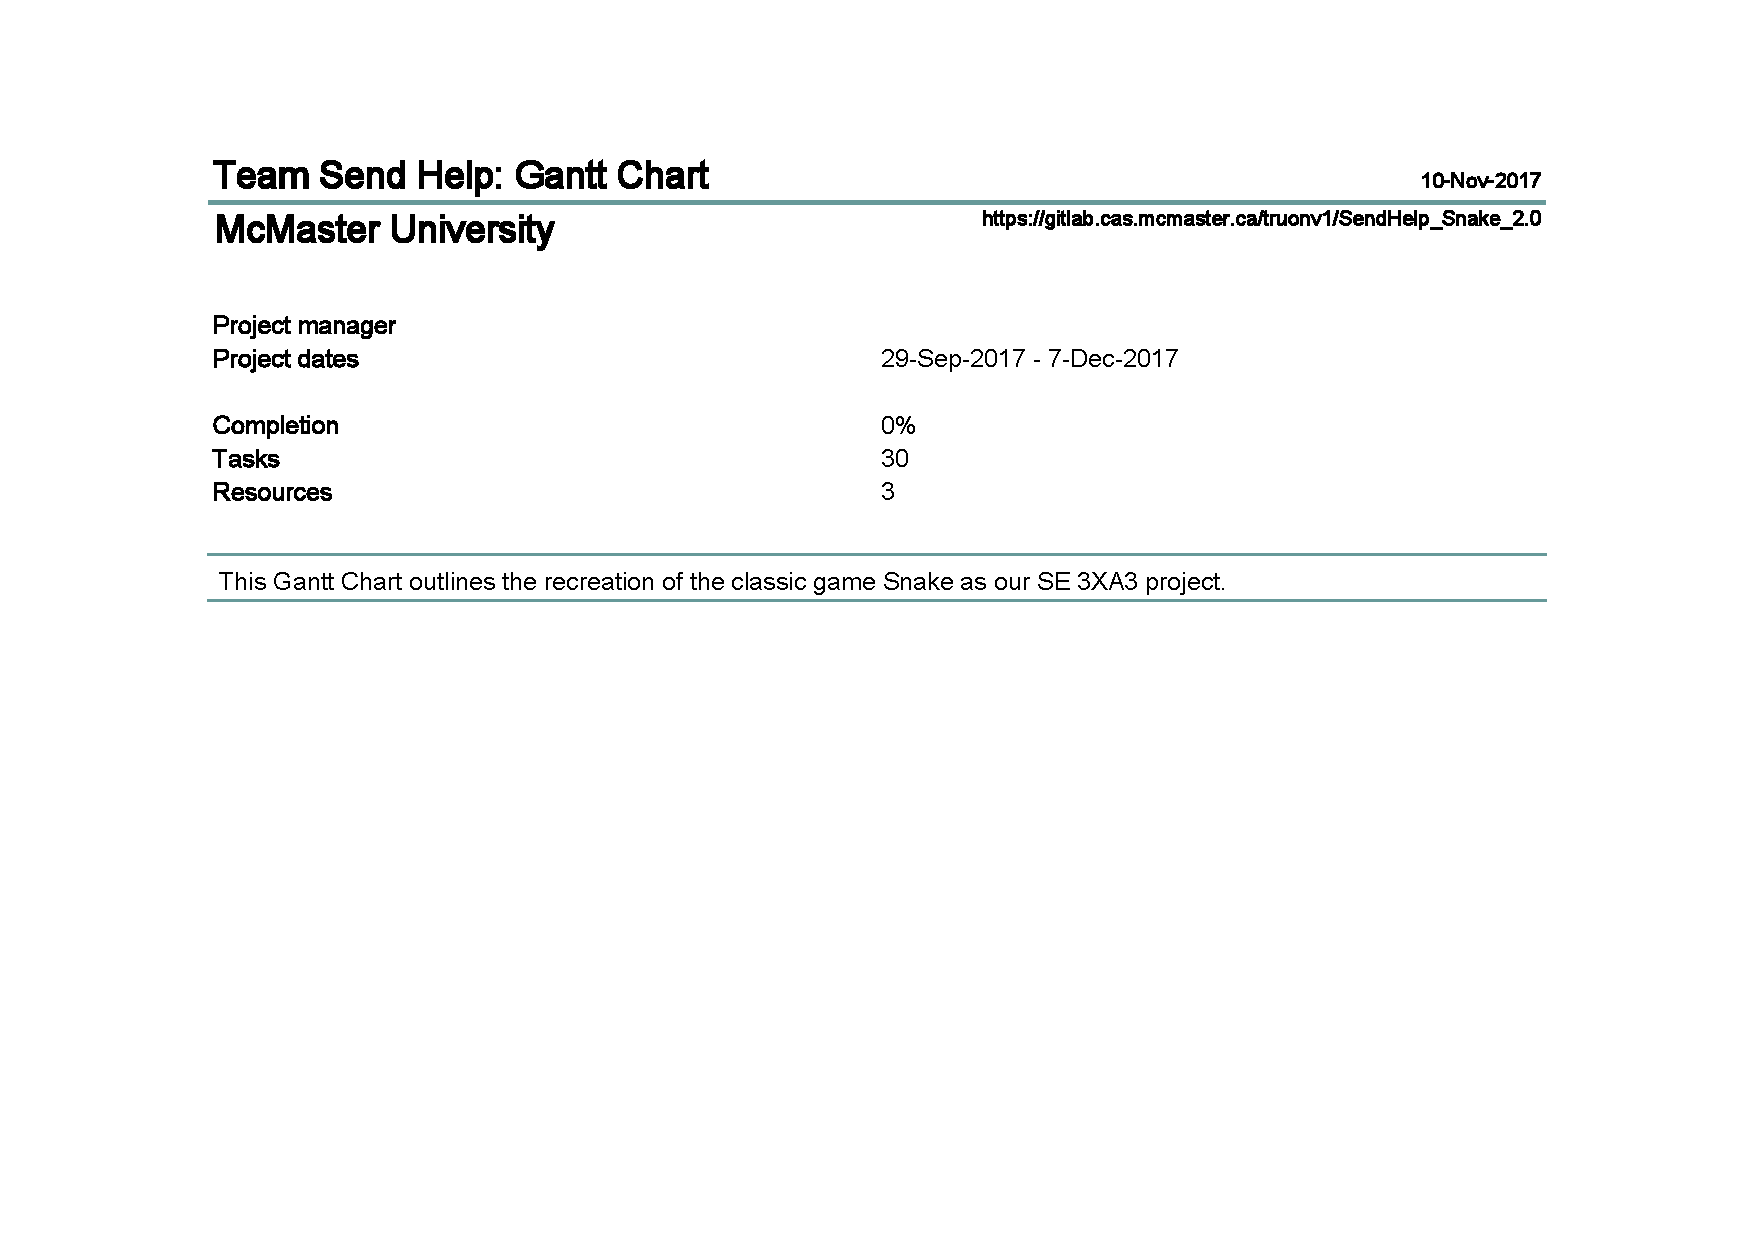
\includepdf[pages={-}]{SendHelp_ganttchart.pdf}

%\section*{References}

\bibliographystyle {plainnat}
\bibliography {MG}

\end{document}
